\documentclass[a4paper,10pt,twoside]{article}
\usepackage[utf8]{inputenc}
\usepackage[french]{babel}
\usepackage[T1]{fontenc}
\usepackage{amsmath}
\usepackage{amsfonts}
\usepackage{amssymb}
\usepackage{graphicx}
\usepackage{multicol}
\usepackage{array}
\usepackage{float}
\usepackage{epstopdf}
\usepackage[justification=centering]{caption}
\usepackage{caption}
\usepackage{subfig}
\usepackage{gensymb}
\usepackage[bottom]{footmisc}
\usepackage{appendix}
\usepackage{pdfpages}
\usepackage{todonotes}
\usepackage{mathpazo}
\usepackage{titleps}
\usepackage{color}
\usepackage{hyperref}
\usepackage[skins]{tcolorbox}
\usepackage{sectsty} 
\usepackage[arrowmos]{circuitikz}
\usepackage{pgfplots}
\usepackage{blindtext}
\usepackage{adjustbox}
\usepackage{listings}
\usepackage[inner=2.5cm,outer=2.5cm,top=3cm,bottom=3cm]{geometry}

\graphicspath{{pictures/}}
\setlength\parindent{0pt}
\renewcommand*\rmdefault{ppl}
\newcolumntype{C}[1]{>{\centering\let\newline\\\arraybackslash\hspace{0pt}}m{#1}}
\newcolumntype{R}[1]{>{\raggedright\arraybackslash}p{#1}}
\sectionfont{\large}
\subsectionfont{\normalsize}

% Page style definitions
\newpagestyle{main}{
	\sethead[Club ELEC : Quête de la balise RF][][]  % even
			{\chaptertitle}{}{Club ELEC : Quête de la balise RF}
	\headrule
    \setfoot[\thepage][][]
    		{}{}{\thepage}		
}

\newpagestyle{appendix}{
	\sethead[Club ELEC : Annexes][][]  % even
			{}{}{Club ELEC : Annexes}
	\headrule
    \setfoot[\thepage][][]
    		{}{}{\thepage}
    \footrule
}

%----------------------------------------------------------------------------------------
%	TITLE SECTION
%----------------------------------------------------------------------------------------
\title{	
	\vspace{2.5cm}
	\normalfont \normalsize 
	\huge Club ELEC\\ 
	\huge Quête de la balise RF de LLN\\
	\huge Phase 2 - Programmation
	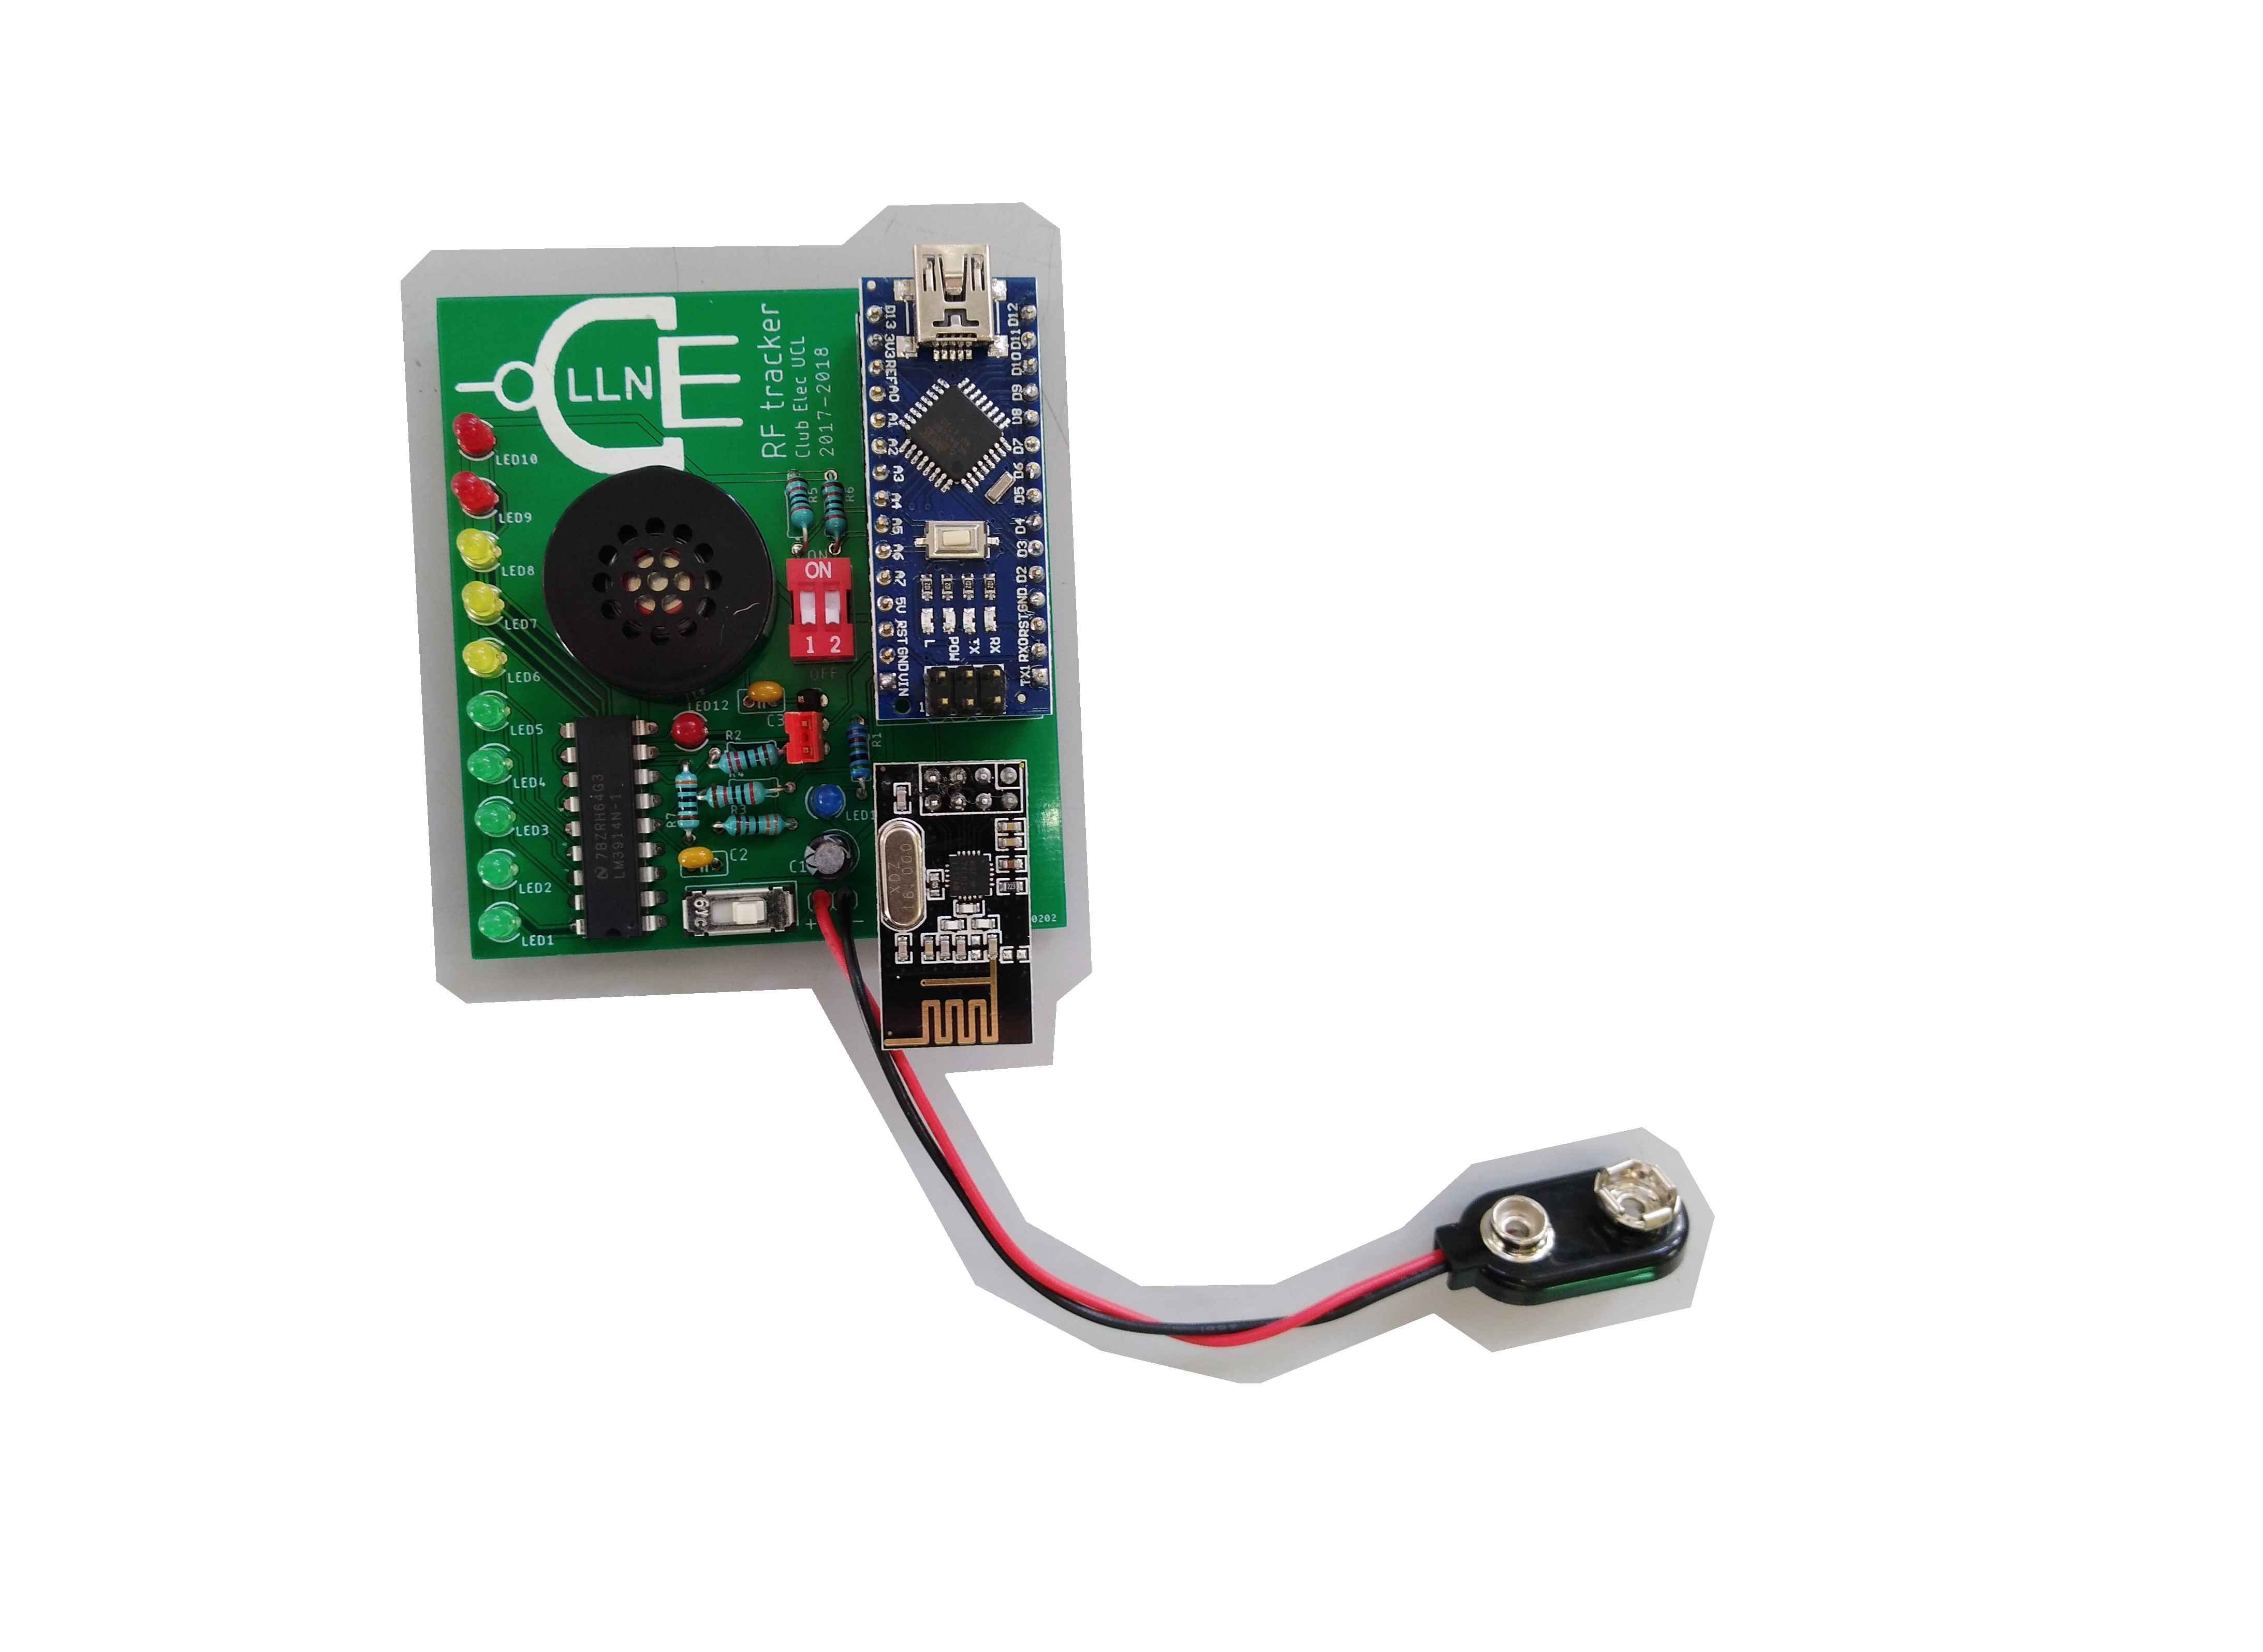
\includegraphics[width=.9\textwidth]{imgs/RF_TAG_withoutBackground.jpg}
	\vspace{2.5cm}
	\centering
}

\begin{document}
\renewcommand{\figurename}{Fig.}
\renewcommand{\thepage}{\roman{page}}
\setcounter{page}{1}

\pagenumbering{gobble}
\maketitle
\newpage
\pagenumbering{arabic}
\pagestyle{main}

\newpage
\null
\thispagestyle{empty}
\newpage
\clearpage

\setcounter{page}{1}

%%% Introduction
\section*{La Quête de la balise RF perdue dans Louvain-la-Neuve}

Bienvenue au Club ELEC pour le projet de ce quadrimestre, à savoir la \textit{Quête de la balise RF de Louvain-la-Neuve}! Nous avons besoin de vous! En effet, une \textbf{balise RF émettrice} a été perdue dans la ville de Louvain-la-Neuve. Votre mission, si vous l'acceptez? La localiser.\\ 

Pour accomplir cette mission, vous aurez tout d'abord besoin d'une ... \textbf{balise RF réceptrice}. À l'aide de celle-ci, vous pourrez correctement réceptionner les messages transmis par la balise perdue et la retrouver les premiers!
\\

Concrètement, le projet à réaliser sera subdivisé en 3 phases:\\
\begin{itemize}
	\item[$\bullet$] Phase 1: compréhension et assemblage de la balise RF réceptrice;
	\item[$\bullet$] Phase 2: programmation de la balise RF réceptrice;
	\item[$\bullet$] Phase 3: localisation de la balise RF perdue. \newline
\end{itemize}

Aujourd'hui, nous attaquons la \textbf{phase 2} de cette quête. L'objectif est de programmer correctement votre balise RF réceptrice, afin de pouvoir recevoir correctement les messages émis par la balise RF émetrice. Le module central de votre balise est la plateforme Arduino Nano. Celle-ci peut être vu comme le "cerveau" de votre carte  électronique, et c'est cette plateforme que vous allez apprendre à programmer.

\begin{center}
Bonne lecture, et puisse le sort vous être favorable!
\end{center}

%%% Installations
\section{Installations nécessaires}
Avant de pouvoir programmer votre balise réceptrice, plusieurs étapes sont nécessaires. 

Il vous faut d'abord \textbf{télécharger et installer le programmateur Arduino}. Celui-ci est aussi appelé Arduino IDE (Arduino Integrated Development Environment). Voici les instructions à suivre :
\begin{enumerate}
	\item se rendre sur la page principale du site Arduino (\url{www.arduino.cc/}) ;
	\item cliquer sur l'onglet "Software" ; 
	\item choisir votre version d'Arduino IDE (voir Fig. \ref{fig:arduino_ide}) et la télécharger ;
	\item une fois le téléchargement effectué, il ne vous reste plus qu'à installer le programmateur.
\end{enumerate}

\begin{figure}[ht!]
	\centering
	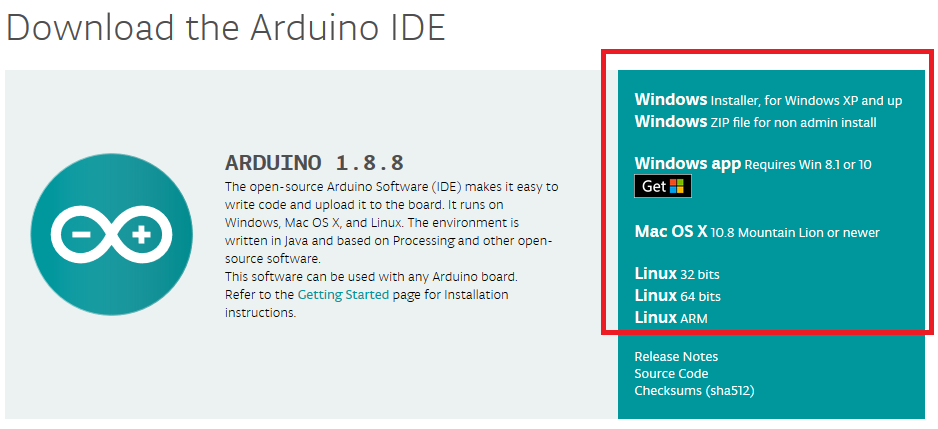
\includegraphics[width=\textwidth]{imgs/arduino_ide.png}
	\caption{Téléchargement du programmateur Arduino.}
	\label{fig:arduino_ide}
\end{figure}

Patience, avant de programmer il vous reste encore quelques étapes. En effet, une fois l'IDE installé, il vous faudra également \textbf{installer la librairie RF24}. Celle-ci permettra à votre module Arduino Nano de communiquer correctement avec le module RF qui y est connecté . Voici les instructions à suivre :
\begin{enumerate}
	\item ouvrir l'Arduino IDE fraichement installé ;
	\item aller dans \textit{Sketch --> Include Library --> Manage Libraries...} ;
	\item taper "RF24" dans la barre de recherche ;
	\item cliquer sur la librairie "RF24" (voir Fig. \ref{fig:arduino_RF24}) et l'installer ;
	\item voilà ! 
\end{enumerate}

\begin{figure}[ht!]
	\centering
	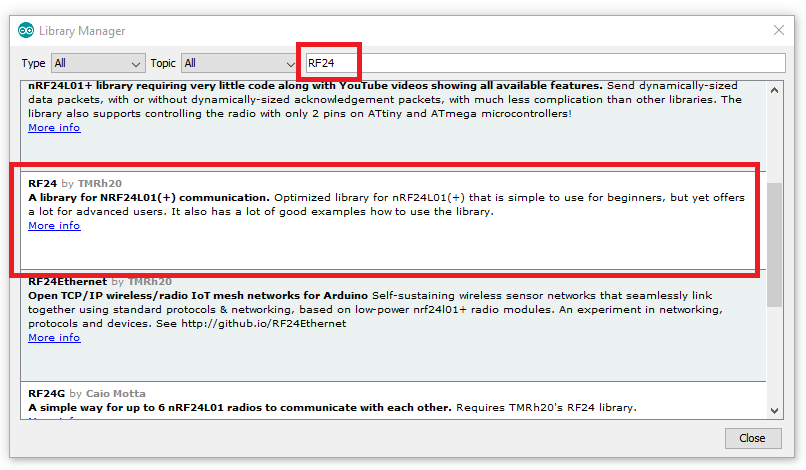
\includegraphics[width=\textwidth]{imgs/arduino_RF24.png}
	\caption{Installation de la librairie RF24.}
	\label{fig:arduino_RF24}
\end{figure}

Vous êtes enfin prêts à programmer votre module Arduino. Vous l'aurez remarqué, Arduino est open-source et gratuit. Sachez aussi qu'il existe une floppée de librairies existantes pour faire à peu près n'importe quoi !
 
%%% Principe de fonctionnement
\section{Votre premier programme Arduino !}
Pour vous aider à vous lancer dans le fabuleux monde de la programmation Arduino, voici quelques instructions pour lancer le code exemple pour votre baliser RF réceptrice. 

\subsection{Configurations}
Il y a d'abord quelques étapes préliminaires :
\begin{enumerate}
	\item ouvrir l'Arduino IDE ;
	\item brancher le module Arduino à votre PC via un câble USB ;
	\item copier le code qui se trouve dans le fichier \textit{reception} fourni dans l'IDE ; 
	\item sauver le croquis (Sketch en anglais) en allant dans \textit{File --> Save} ou simplement en appuyant sur \textit{CTRL + S} ;	
\end{enumerate}

Le résultat devrait être proche de celui de la Fig. \ref{fig:arduino_reception}.

\begin{figure}[ht!]
	\centering
	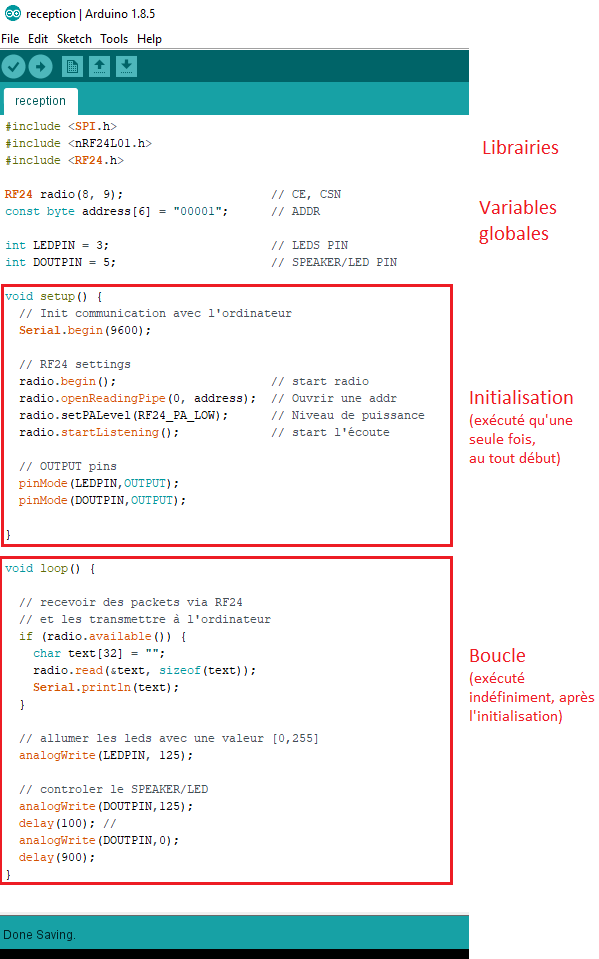
\includegraphics[width=0.6\textwidth]{imgs/arduino_reception.png}
	\caption{Exemple de code récepteur que nous vous fournissons.}
	\label{fig:arduino_reception}
\end{figure}

Avant de programmer le module, il y a encore quelques configurations à effectuer :
\begin{enumerate}
	\setcounter{enumi}{3}
	\item choisir la bonne "board", pour qu'elle corresponde à "Arduino Nano" ; pour cela, aller dans \textit{Tools --> Board --> Arduino Nano} (voir Fig. \ref{fig:arduino_board}) ;
	\item choisir le bon processeur, pour qu'il corresponde à "ATmega328P" ; pour cela, aller dans \textit{Tools --> Processor --> ATmega328P} (voir Fig. \ref{fig:arduino_processor}) ;
	\item choisir le bon port série ; pour cela, aller dans \textit{Tools --> Port} et choisir le port série adéquat (il n'y en a qu'un si vous n'avez qu'une seule connection USB) ;
	\item voilà, il est temps de programmer votre module Arduino ; il suffit de cliquer sur \textit{Sketch --> Upload} ou d'utiliser \textit{CTRL + U}.
\end{enumerate}

\begin{figure}[ht!]
	\centering
	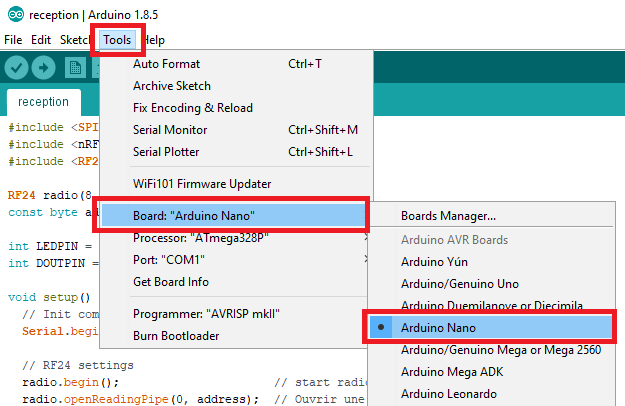
\includegraphics[width=0.6\textwidth]{imgs/arduino_board.png}
	\caption{Configuration de la "board".}
	\label{fig:arduino_board}
\end{figure}

\begin{figure}[ht!]
	\centering
	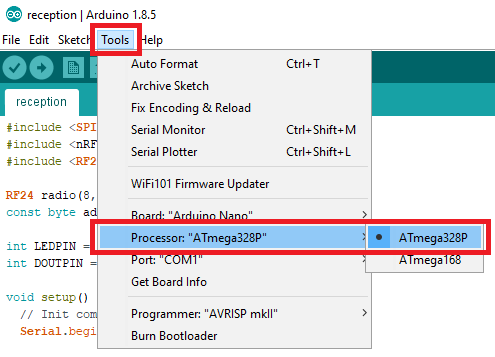
\includegraphics[width=0.6\textwidth]{imgs/arduino_processor.png}
	\caption{Configuration du processeur.}
	\label{fig:arduino_processor}
\end{figure}

Si tout se passe bien, votre carte électronique devrait faire de jolies choses ! 

\newpage
\subsection{Explication du code}
Maintenant que votre carte est programmée, il est important de comprendre ce qu'elle fait. Pour cela, il suffit de comprendre le code repris à la Fig. \ref{fig:arduino_reception}. Le code est structuré en plusieurs parties, comme repris sur la figure :
\begin{enumerate}
	\item d'abord, on inclut les \textbf{librairies} utiles ; dans notre cas, la librairie "RF24", qui a besoin également de deux autres librairies ;
	\item ensuite, on définit plusieurs \textbf{variables globales} ; par exemple, \texttt{LEDPIN = 3} indique que la pin 3 de l'Arduino est utilisée pour allumer les LEDs, via le LED driver ; 
	\item la fonction \texttt{setup} sert d'\textbf{initialisation} et n'est exécutée qu'une seule fois, au tout début (quand on branche l'alimentation par exemple) ; dans cette fonction :
		\begin{itemize}
			\item le moniteur série est configuré (ce dernier permet d'envoyer du texte à l'ordinateur ; pour l'activer, il suffit d'aller dans \textit{Tools --> Serial Monitor}) ;
			\item la radio est configurée (canal, adresse, etc.) ;
			\item les pins de sortie de l'Arduino sont configurées (LEDs et buzzer) ;
		\end{itemize}
	\item enfin, la fonction \texttt{loop} est la \textbf{partie centrale du code} ; cette fonction est exécutée indéfiniment après la phase d'initialisation ; dans le code d'exemple :
		\begin{itemize}
			\item on attend de recevoir un message et on le transmet vers l'ordinateur via le port série ;
			\item on allume les LEDs via le LED driver ;
			\item on allume la LED seule ou le buzzer pendant un petit moment.
			\item et on recommence la fonction \texttt{loop} !
		\end{itemize}			
\end{enumerate}
	
\section{Conclusion}
À partir de maintenant, vous pouvez partir du code exemple et le modifier à votre guise. Votre tâche est de recevoir correctement les messages émis par la balise émetrice pour pouvoir la localiser correctement. 

Voici quelques derniers conseils pour mener à bien votre mission:
\begin{itemize}
	\item nous vous avons fourni le code de l'émetteur (fichier \textit{transmit}) ; nous vous conseillons de bien le comprendre pour mettre en place votre stratégie de localisation ! 
	\item quand vous utilisez les pins de l'Arduino, pour par exemple allumer une LED, vérifiez toujours que cette LED est bien connectée à la pin que vous choisissez dans le code.
	\item posez des questions, n'hésitez surtout pas, nous sommes là pour cela !
\end{itemize}

\begin{center}
Que la force soit avec vous !
\end{center}

\end{document}